

%%%%%%%%%%%%%%%%%%%%%%%%%%  PREAMBLE

\documentclass{beamer}
\usetheme{Singapore}
%\usecolortheme{beaver}

% Load Packages
\usepackage{graphicx}
\usepackage{tikz}
\usepackage{caption}
\usepackage{bm}
\usepackage{xcolor}

% Biblio/References
\usepackage[backend=biber,style=apa,sorting=nyt]{biblatex}
\renewcommand*{\bibfont}{\scriptsize}     % Make the bibliography text smaller
\addbibresource{biblio.bib} % Point to your .bib file

% Avoid "Figure" in the Figure Caption
\captionsetup[figure]{labelformat=empty}

% Title page info
\title[Research Methods in WOP - AIP Young Keynote]{Research Methods in Work and Organizational Psychology: Towards an Integration Between Theory-driven and Data-driven Modeling}
\subtitle{Young Keynote Speaker}
\author{Enrico Perinelli}
\institute{Department of Psychology and Cognitive Science \\ University of Trento}
\date{September 4, 2024}

% Table of contents at the beginning of each section and shaded
\AtBeginSection[]{
    \begin{frame}{}
        \tableofcontents[currentsection, sectionstyle=show/shaded, subsubsectionstyle=show/shaded/hide]
    \end{frame}
}

%%%%%%%%%%%%%%%%%%%%%%%%%%  START DOCUMENT

\begin{document}


%%%%%%%%%%%%%%%%%%%%%%%%%% Title page

\begin{frame}
    \titlepage
    \begin{center}
    \begin{tikzpicture}[remember picture, overlay]
        % Left image
        \node[opacity=1, inner sep=1pt] at ([xshift=2.2cm,yshift=2.2cm]current page.south west) {
            
\includegraphics[height=0.1\paperheight]{figs/logoDIPSCO.png}
        };
        % Right image
        \node[opacity=1, inner sep=1pt] at ([xshift=-2.2cm,yshift=2.2cm]current page.south east) {
            
\includegraphics[height=0.1\paperheight]{figs/logoAIP.png}
        };
    \end{tikzpicture}
    % Horizontal line with margins (this entails the whole space possible, since the \rule parameter set to `1`; for this reason, do not use `\\` to change the line after drawing the line, otherwise it creates too space)
    \hspace{0\linewidth}\rule{1\linewidth}{0.2pt}
    \begin{tiny}
        Immaginazione organizzativa, ricerca e azione trasformativa. Passato, presente e futuro delle pratiche di psicologia del lavoro e delle organizzazioni\\
        XX Congresso Nazionale della Sezione di Psicologia per le Organizzazioni\\
        Bergamo, 4-5-6 Settembre 2024
    \end{tiny}
    \end{center}
\end{frame}


%%%%%%%%%%%%%%%%%%%%%%%%%% TOC

\begin{frame}{Table of Contents}
    \tableofcontents
\end{frame}


%%%%%%%%%%%%%%%%%%%%%%%%%% Intro

\section{Intro}


\begin{frame}{Preamble}
    \setbeamercovered{transparent}
    \begin{itemize}
        \item<1> Work and Organizational Psychology (WOP) encompasses a wide range of research and applied areas, exploring the intersections between individuals, groups, organizations, jobs, and policies.
        \item<2> According to \textit{Journal Citation Reports}, there are \textbf{114} scientific journals categorized under ``PSYCHOLOGY, APPLIED'' and \textbf{403} under ``MANAGEMENT''
        \item<3> Some of you specialize in:
            \begin{itemize}
                \item Leadership Studies... others may not
                \item Individual Differences... others may not
                \item Safety at Work... others may not
                \item Occupational Health... others may not
                \item Vocational Behaviors... others may not
                \item Human Resources Management... others may not [...]
            \end{itemize}
        \item<4> Despite these diverse specializations, we all dedicate significant time to \color{red}{\textbf{Research Methods}}.
    \end{itemize}
\end{frame}


\begin{frame}{Research Methods in WOP}
    \begin{columns}[t] % [t] aligns the content at the top of each column
        
        % Left column (1/3 of the width)
        \column{0.67\textwidth}
        % Content for the left column goes here
        \begin{itemize}
            \item The adoption of advanced research methods and data analyses is becoming more and more important for conducting high-quality research in WOP
            
            \item Whole journal: \textit{Organizational Research Methods} {\scriptsize (Academy of Management \textemdash  \textit{Research Methods} Division)}
            
            \item Book: \textcite{landers2024}
            
            \item Growing number of books and special issues on HR Analytics
            \scriptsize \parencite[]{bauer2024HR, caughlin2024r, edwards2024hr, khan_milner2023, mcnulty2022handbook, starbuck2023fundamentals}    
        \end{itemize}

        % Right column (2/3 of the width)
        \column{0.33\textwidth}
        \vspace{-1cm} % Adjust this value as needed to move the figure up
        \begin{figure}
                \centering
                
\includegraphics[width=1.1\linewidth]{figs/Landers_cover.png}
            % \caption{Enter Caption}
            \label{fig:Landers}
        \end{figure}
    \end{columns}
\end{frame}


\begin{frame}{Qualitative and Quantitative (well-known) Distinction}
    Two macro-areas in WOP Research Methods
    \begin{itemize}
        \item \textbf{Qualitative Research:} ``[r]esearch focused on deep understanding and narrative description; typically involve collection of unstructured data and tends to be more exploratory''\begin{footnotesize}\parencite[p. 443]{landers2024}\end{footnotesize}    
        \item \textbf{Quantitative Research:} ``[r]esearch focused on careful measurement and precision to capture information about constructs; typically relies on statistics''\begin{footnotesize}\parencite[p. 443]{landers2024}\end{footnotesize}
    \end{itemize}
\end{frame}

\begin{frame}{Philosophical (less-known...) Foundations}
    \begin{figure}
        \centering
        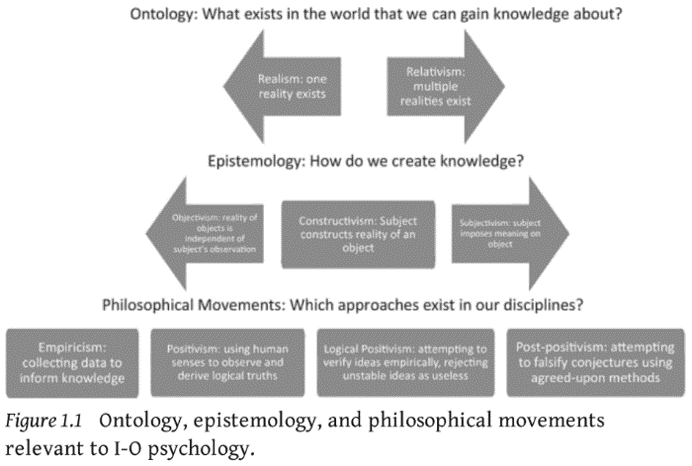
\includegraphics[width=0.9\linewidth]{figs/Philosopical.png}
        \caption{{\small Source: \textcite[p. 5]{landers2024}.\\See also Chapter 6 in \textcite{braun2022thematic} for a thorough discussion on philosophical foundations in empirical research}}
        \label{fig:philos}
    \end{figure}
\end{frame}


\begin{frame}
\frametitle{Epistemology in Quant Research}
\framesubtitle{Theory-Driven vs Data-Driven Modeling}
\setbeamercovered{transparent}
    \begin{itemize}
        \item<1-2>  \textbf{Theory-driven} modeling
            \begin{itemize}
                \item<1-2>  \textit{Approach:} Hypothetico-deductive (from theory to data)
                \item<1-2> \textit{Label:} Confirmatory
                \item<1-2> \textit{Aim:} Explanation
            \end{itemize}
        \item<1-2> \textbf{Data-driven} modeling
            \begin{itemize}
                \item<1-2> \textit{Approach:} Inductive (from data to insights)
                \item<1-2> \textit{Label:} Exploratory
                \item<1-2> \textit{Aim:} Prediction
            \end{itemize}
        \item<2-> In \textbf{Statistics}, this debate has at least two decades\begin{scriptsize}
            \parencite[]{breiman2001, shmueli2010}
        \end{scriptsize}
        \item<2-> In \textbf{Psychology}, it's rather new\begin{scriptsize} \parencite[]{yarkoni2017,jacobucci2022, paxton2017} \end{scriptsize}
        \item<2-> In \textbf{WOP and Management} it's even newer\begin{scriptsize} \parencite[]{leavitt2021, woo2024} \end{scriptsize}
    \end{itemize}
\end{frame}


\begin{frame}{Towards a paradigm shift?}
    \begin{figure}
        \centering
        
\includegraphics[width=0.9\linewidth]{figs/wop_psychom_dataScience.png}
        \caption{Integration between WOP and two methodological areas}
        \label{fig:wop_psychom_dataScience}
    \end{figure}
\end{frame}


%%%%%%%%%%%%%%%%%%%%%%%%%% Theory-driven

\section{Theory-driven modeling in WOP}

\begin{frame}{Theory in WOP}
    \begin{quote}
        \small
        \textit{``Management and organizational scholars have defined theory in similar ways over the past several decades. For example, Davis (1971); Bacharach (1989); Whetten (1989); Weick(1995); Sutton and Staw (1995); Alvesson and Sandberg (2011); Ragins (2012); Bettis, Gambardella, Helfat, and Mitchell (2014); Suddaby (2014); Cornelissen (2017); and van Nordenflicht (2023), among others, focus on concepts, relationships, assumptions, boundary conditions, consistency, parsimony, and falsifiability.\\ \textbf{Drawing from these articles and other salient sources, we define theory as an explanation of the relationships between constructs or concepts that show how and why a phenomenon occurs.}''}
        \begin{flushright}
            \scriptsize
            \parencite[p. 1183-1184]{thatcher2024_JOM}
        \end{flushright}
    \end{quote}
\end{frame}


\begin{frame}{Hypothesis in WOP}
    \begin{quote}
        \small
        \textit{``Many investigations go beyond raising questions by stating specific theoretical hunches, or hypotheses, about the outcomes of a study. \textbf{A hypothesis is the researcher’s best guess about what the results of a study will be.} Rather than merely raising the question, the hypothesis is a theoretical answer. \\ Thus, one might hypothesize that `People who are well paid will like their jobs better than people who are not.'\\ or\\ `People who are fairly paid will like their jobs more than people who are not.'\\ \textbf{The hypothesis is a statement of the results that the researcher expects to find.} Research studies are conducted to \textbf{\underline{confirm}} hypotheses. In other words, do the results come out the way they were predicted?''}
        \begin{flushright}
            \scriptsize
             \parencite[p. 25]{spector2017}
        \end{flushright}
    \end{quote}
\end{frame}


\begin{frame}{}
Tell me how important theory is in WOP without telling me how important theory is in WOP...
    \begin{figure}
        \centering
        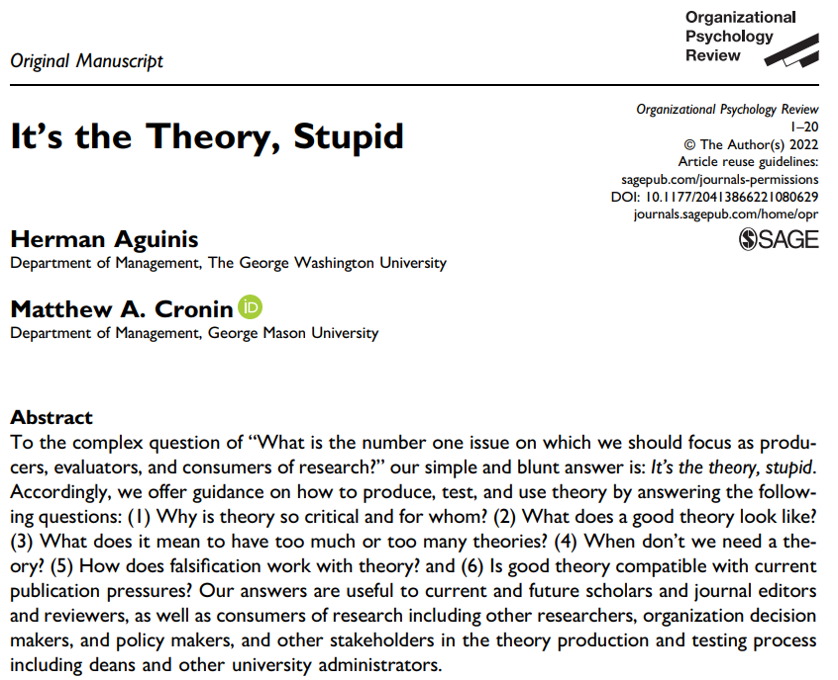
\includegraphics[width=0.75\linewidth]{figs/Aguinis_theoryOPR.png}
        \caption{Source: \textcite[]{aguinis_theoryOPR}}
        \label{fig:enter-label}
    \end{figure}
\end{frame}


\begin{frame}{Why theory is so important in WOP?}
	\small
	We need a thorough knowledge of WOP phenomena to
	\begin{enumerate}
	    \item Measure variables that are not directly measurable (i.e., constructs)
	    \item Connect constructs to unravel complexities in their relationship
	\end{enumerate}
	In this scenario, two areas of Psychometrics are essential for translating, testing, validating, and expanding WOP theories into empirical findings.
	\begin{enumerate}
	    \item Psychological Assessment/Measurement (e.g., operationalization process, reliability, validity) {\scriptsize \parencite[e.g.,][]{cheung2024validity}}
	    \item Data Analytic Techniques (e.g., G(z)LM, mediation/moderation, multilevel modeling, Structural Equation Modeling, person-centered approaches) {\scriptsize \parencite[e.g.,][]{gonzalez2023mlm, morin2018person_centered}}
	\end{enumerate}
\end{frame}


\begin{frame}{Substantive-Methodological Synergy}
	\setbeamercovered{transparent}
	\begin{itemize}
	    \item<1> Originally developed in Psychometrics \parencite[e.g.,][]{borsboom2006} to enhance the exchange between substantive psychological areas and psychometric methods
	    \item<2-> Now also widely adopted in WOP, as outlined by \textcite[]{hofmans2021} in a \textit{I-O Psych} paper titled   ``\textit{The baby and the bathwater: The need for substantive–methodological synergy}''. Main points: 
	    \begin{itemize}
	        \item<3> The importance of methodological fit
	        \begin{itemize}
	            \item Many phenomena in I-O psychology are multidetermined
	            \item Much of our data have a nested data structure
	            \item Psychological phenomena are usually dynamic
	            \item The questionable assumption of population homogeneity
	            \item Many theories, even simple in appearance, cannot be empirically tested without complex data analyses
	        \end{itemize}
	        \item<4> The need for latent variable models
	        \begin{itemize}
	            \item Random measurement error
	            \item Disentangling distinct sources of variance
	            \item Improved techniques for testing moderation
	        \end{itemize}
	        \end{itemize}
	    \end{itemize}
\end{frame}


\begin{frame}
\frametitle{Operationalization process in WOP}
\framesubtitle{What we do when we operationalize a construct in WOP?}
	\begin{figure}
		\centering
		\only<1>{
			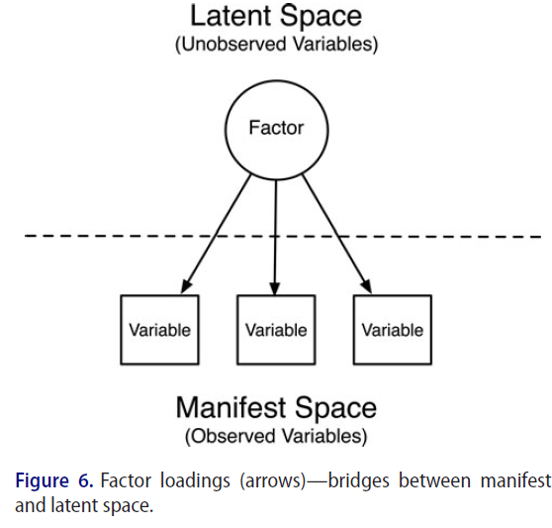
\includegraphics[width=0.6\linewidth]{figs/Nesserl_moleenar_2016.png}
			\caption{Source: \textcite[p. 404]{nesselroade2016}}
			\label{fig:nesserl}
		}
		\only<2>{
			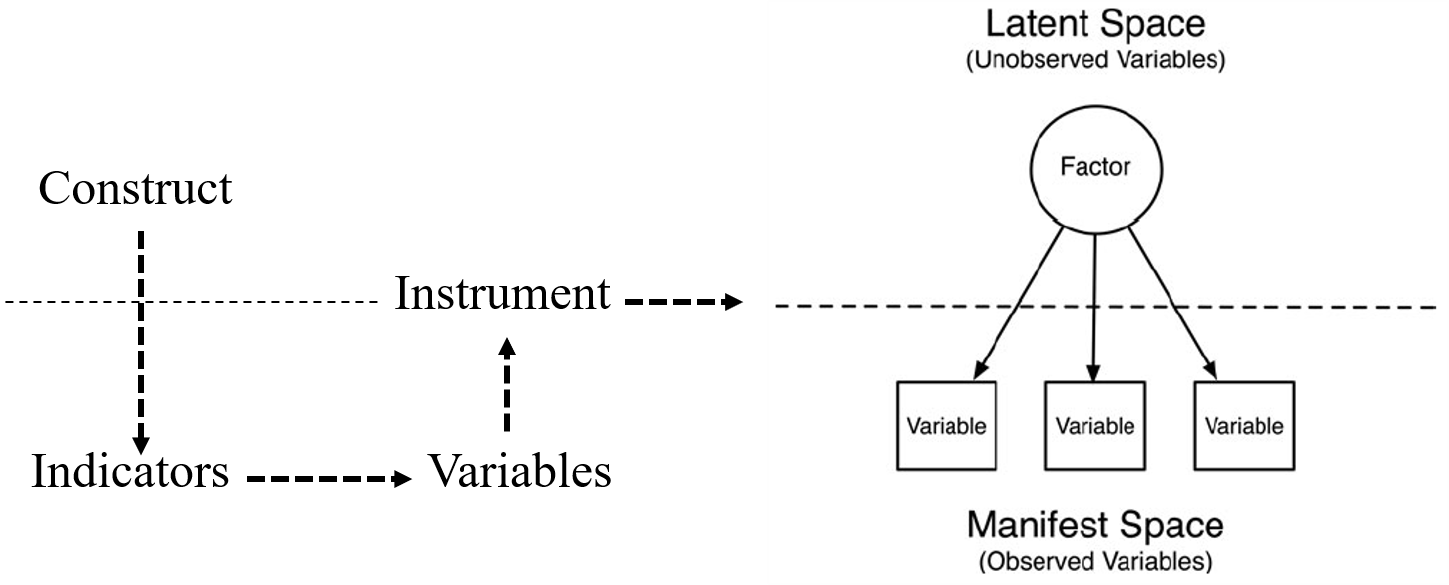
\includegraphics[width=1\linewidth]{figs/operaz_process1.png}
			% \caption{} 
			\label{fig:operaz1}
		}
		\only<3>{
			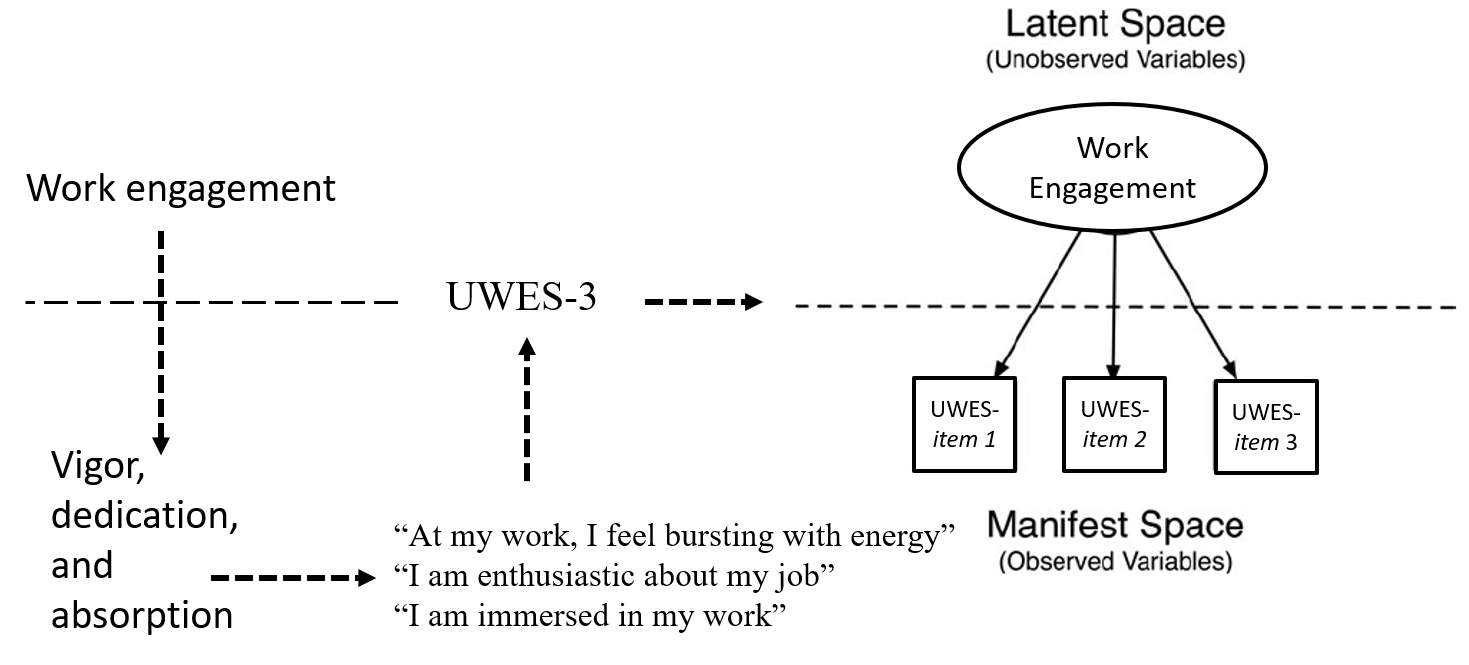
\includegraphics[width=1\linewidth]{figs/operaz_process2_uwes.png}
			\caption{Source of UWES-3: \textcite[]{schaufeli2017uwes}}
			\label{fig:operaz2}
		}
	\end{figure}
\end{frame}


\begin{frame}
\frametitle{Operationalization process in WOP}
\framesubtitle{What we do when we operationalize a construct in WOP?}
	Validity in WOP:
	\begin{itemize}
		\item Substantive Validity
		\begin{itemize}
			\item Face Validity {\scriptsize \parencite{allen2023face}}
			\item Content Validity {\scriptsize \parencite{colquitt2019content, rossiter2008content}}
		\end{itemize}
		\item Structural (Internal) Validity
		\begin{itemize}
			\item Reliability {\scriptsize \parencite{cortina2020alpha}}
			\item Measurement Invariance {\scriptsize \parencite{somaraju2022measurInvar}}
		\end{itemize}
		\item External Validity
		    \begin{itemize}
		    	\item Construct/Nomological/Criterion Validity {\scriptsize \parencite[e.g.,][]{lambert2023ConstrVal}}
		    	\item Convergent Validity {\scriptsize \parencite{cheung2024validity}}
		    	\item Discriminant Validity {\scriptsize \parencite{cheung2024validity, ronkko2022}}
		\end{itemize}
	\end{itemize}	
\end{frame}


\begin{frame}
	\frametitle{Structural relationships among WOP constructs}
	\framesubtitle{What we do when we connect constructs in WOP?}
	
	\begin{itemize}
		\item Test theory against data using Structural Equation Modeling
        \item Theory guides the way to which we specify a certain degree of misfit ($\mathbf{\Sigma(\Theta)}$) in original data (\(\mathbf{\Sigma}\))
        \item Will data support theory, i.e. will $\mathbf{\Sigma} = \mathbf{\Sigma}(\bm{\Theta})$?{\scriptsize \parencite{bollen1989}}
    \end{itemize}
 
 \begin{figure}[htbp]
 	\centering
 	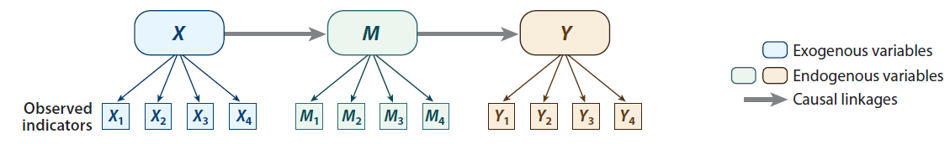
\includegraphics[width=1.05\linewidth]{figs/zyphurSEM.png}
 	\caption{Source: \textcite[p. 497]{zyphur2023structural}}
 	\label{fig:sem}
 \end{figure}
\end{frame}


\begin{frame}
	\frametitle{Structural relationships among WOP constructs}
	\framesubtitle{What we do when we connect constructs in WOP?}
	
	\textbf{The pivotal contribution of Longitudinal SEM}
	
	\only<1>{
	\begin{itemize}
		\item Mostly based on \textit{Granger causality} from econometrics {\scriptsize \parencite{granger1969}} 
		\item Improved test of mediation hypotheses {\scriptsize \parencite{aguinis2017MedMod}}
		\item Track and link mean-level change, autoregression, and various sources of variances (trait, state, state-residual, uniqueness, etc.) of WOP constructs {\scriptsize \parencite[e.g., ][]{zhou2021dsem}}
    \end{itemize}
     }
	
	\only<2->{
	Some substantive-methodological contributions:
	\begin{itemize}
	\setbeamercovered{transparent}
	\item<2-> Global self-esteem at work is not as stable as we thought ... 
		\begin{itemize}
			\item Reject the rigid separation between “state-constructs” and “trait-constructs”
			\item Rather, focus on the trait and state components of each WOP construct {\scriptsize \parencite{perinelli2020lst}}
		\end{itemize}
	\item<3-> Global self-esteem at work is not only a predictor, as we thought ...
		\begin{itemize}
			\item Findings based on the Sociometer Theory support the notion that social environment at work may affect workers' self-esteem levels {\scriptsize (Perinelli, Alessandri, Cepale \& Fraccaroli, \cite*{perinelli2022sociometer})}
		\end{itemize}
	\item<4-> Personality traits are not as stable as we thought ... 
		\begin{itemize}
			\item Instead, adaptability of traits may increase levels of organizational socialization and identification {\scriptsize (Alessandri, Perinelli, Robins, Vecchione, \& Filosa, \cite*{alessandri2020trait})}
		\end{itemize}
	\end{itemize}
	}	
\end{frame}


\begin{frame}
	\frametitle{Theory-driven Modeling in WOP}
	\framesubtitle{Conclusion}
	
	{\scriptsize All the research methods and approaches discussed so far are (and should be treated as) \textbf{DEDUCTIVE}, and thus confirmatory and explanatory
		
    \color{green}{Advantages}
		\begin{itemize}
			\item Ability to test theories against data, from operationalization to structural relationships
			\item Ability to disentangle various sources of variance
			\item Ability to face with complex multivariate issues
		\end{itemize}
	
	\color{red}{Disadvantages}
		\begin{itemize}
			\item Many parameters... but few constructs: {\tiny A 3-wave model with only 3 constructs may require the estimation of more than 150 parameters.}
			\item Difficulties in perfectly fit theory with data and vice-versa: {\tiny What about unexpected findings? What about complex (hidden) non-linearities? What about the effect of other not-controlled variables?}
			\item Over-optimistic estimates of explained variance: {\tiny How well my model fit on future (unseen) data?}
			\item It is difficult to merge Qualitative Research Methods into a single pipeline: {\tiny Mixed-method designs often present qualitative and quantitative methods separately.}
		\end{itemize}}	
\end{frame}


%%%%%%%%%%%%%%%%%%%%%%%%%% Data-driven

\section{Data-driven modeling in WOP}

\begin{frame}
	\frametitle{Data-driven modeling}
%	\framesubtitle{When theory is too much}
	\begin{itemize}
		\item Data-driven models belong to the ``Algorithmic Modeling Culture''
		\item Mid-1980s: Neural nets and decision trees became available
		\item Mainly developed by computer scientists, physicists, and engineers (plus a few aging statisticians)
		\item Complex \textbf{prediction problems} where it was obvious that classical data models were not applicable {\scriptsize (e.g., speech recognition, image recognition, nonlinear time series prediction, handwriting recognition, prediction in financial markets)}
	\end{itemize}
	
	\begin{flushright}
		\textit{\parencite[205]{breiman2001}}
	\end{flushright}
\end{frame}


\begin{frame}
	\frametitle{``Mainstream'' Data-Driven Concepts}
	\begin{figure}
		\centering
		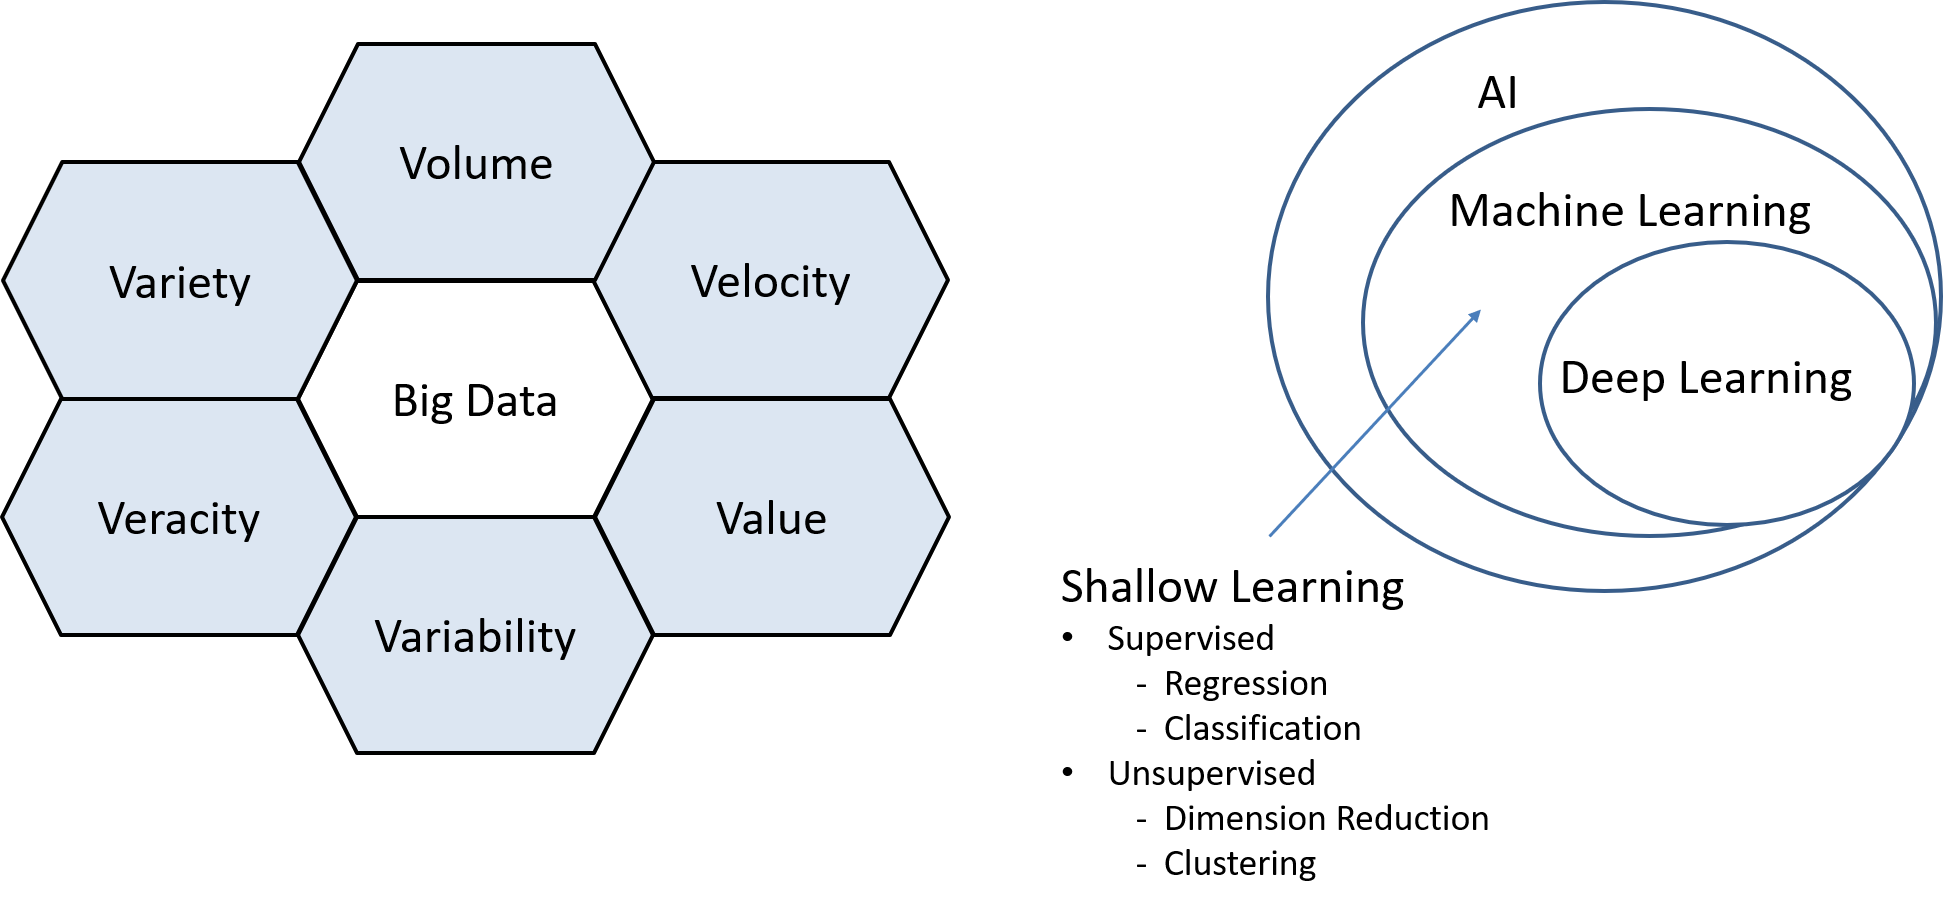
\includegraphics[width=1\linewidth]{figs/BigData_AI.png}
		% \caption{Enter Caption}
%		\label{fig:Landers}
	\end{figure}
\end{frame}

\begin{frame}
	\frametitle{``Less-known'' Data-Driven Concepts}
	\begin{figure}
		\centering
		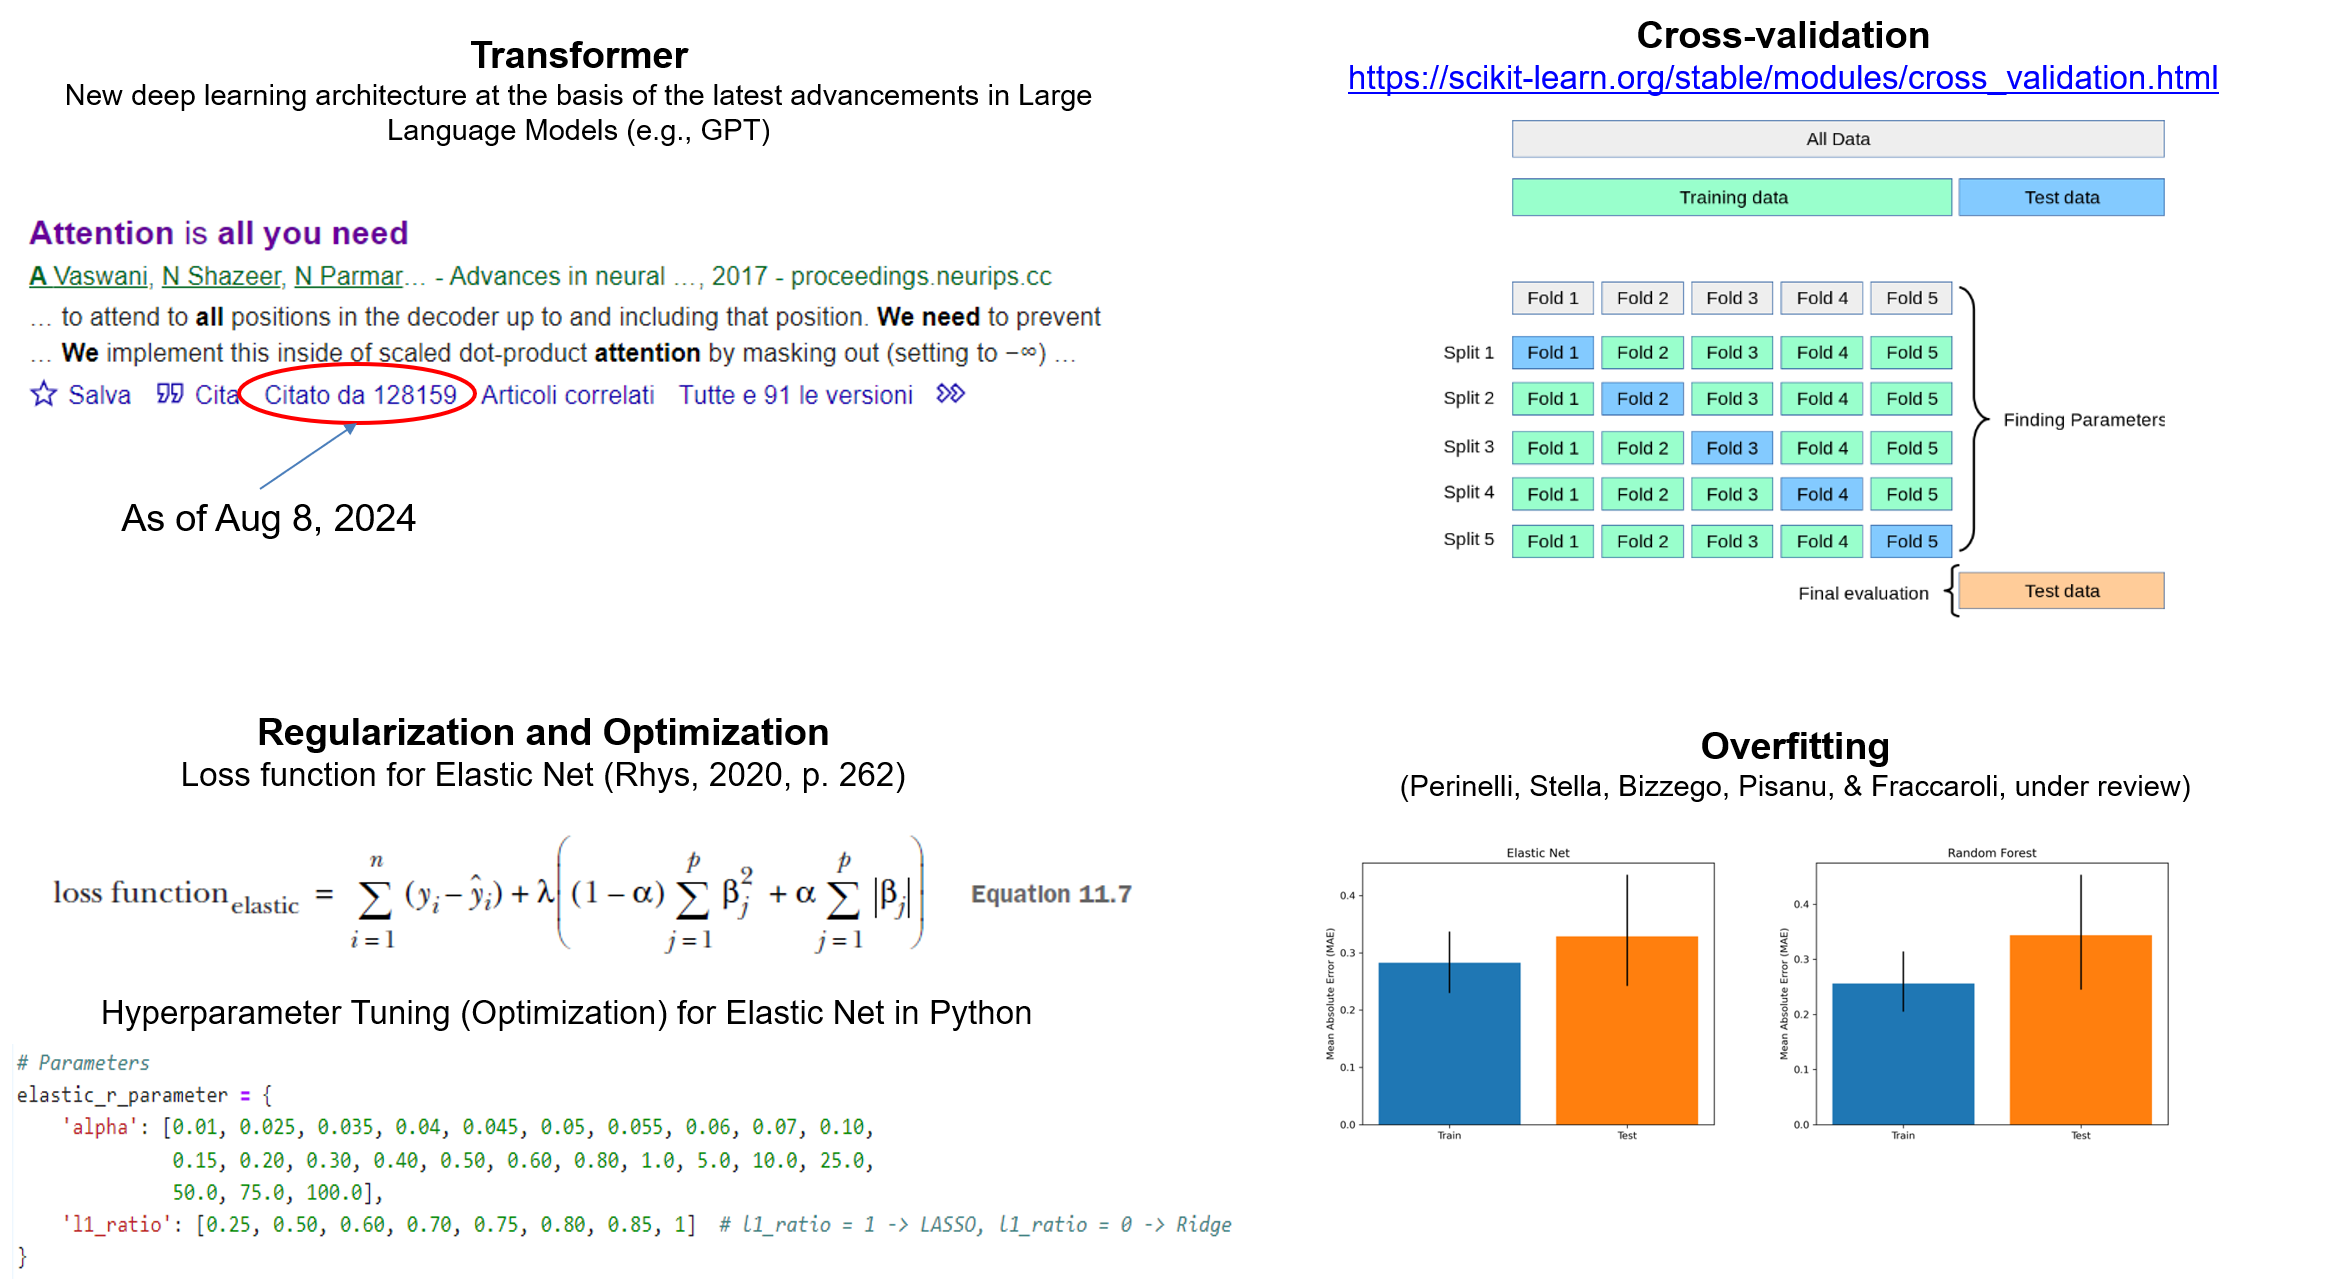
\includegraphics[width=1\linewidth]{figs/BigData_AI_LessKnown.png}
		% \caption{Enter Caption}
%		\label{fig:Landers}
	\end{figure}
\end{frame}

\begin{frame}
	\frametitle{Data-driven Modeling in WOP}
	\begin{itemize}
		\item The first milestones can probably be mapped in a \textit{SIOP Organizational Frontiers Series} book {\scriptsize \parencite{tonidandel2016big}} and in an \textit{ORM} special issue {\scriptsize \parencite{tonidandel2018big}}
		\item Since then:
		\begin{itemize}
			\item 2 special issues on \textit{Personnel Psychology} {\scriptsize \parencite{campion2023machine, woo2024}}
			\item 1 review on the \textit{Annual Review of Org Psych and Org Behav}  {\scriptsize \parencite{oswald2020big}}
			\item Several articles on different topics, such as
			\textbf{leadership} {\scriptsize \parencite{tonidandel2022leadersh}}, 
			\textbf{job analysis} {\scriptsize \parencite{putka2023evaluating}}, 
			\textbf{turnover/performance}  {\scriptsize \parencite{sajjadiani2019using}}, 
			\textbf{work engagement} {\scriptsize \parencite{vanRoekel2024textWorkEngag}},
			\textbf{talent management systems} {\scriptsize \parencite{gonzalez2019talent}}, 
			\textbf{safety outcomes} {\scriptsize \parencite{kumar2024safety}}, 
			\textbf{personnel selection} {\scriptsize \parencite{landers2023simulation, koenig_Tonidandel2023}}, 
			\textbf{tutorial/best practices} {\scriptsize \parencite{putka2018modern, sheetal2023LongitudinalML}}, 
			\textbf{Automatic Item Generation} (AIG) {\scriptsize \parencite{lee2023AIG}}
		\end{itemize}
	\end{itemize}
\end{frame}


\begin{frame}
	\frametitle{Data-driven Modeling in WOP}
	\framesubtitle{Epistemological Considerations}
	\begin{figure}
		\centering
		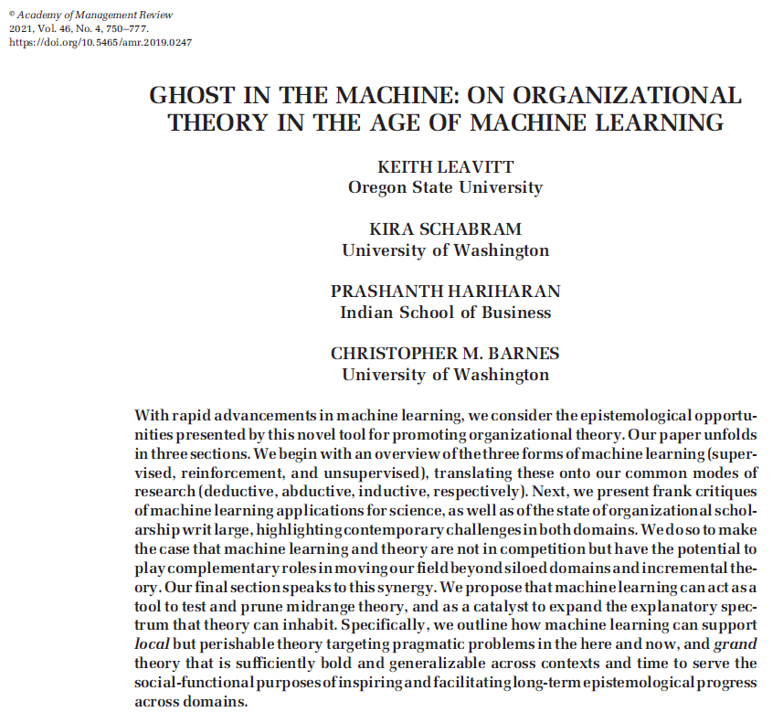
\includegraphics[width=0.6\linewidth]{figs/Leavitt_2021.png}
		\caption{Source: \textcite[]{leavitt2021}}
		\label{fig:leavitt2021}
	\end{figure}
\end{frame}


\begin{frame}
	\frametitle{Data-driven Modeling in WOP}
	\framesubtitle{Epistemological Considerations}
	\begin{figure}
		\centering
		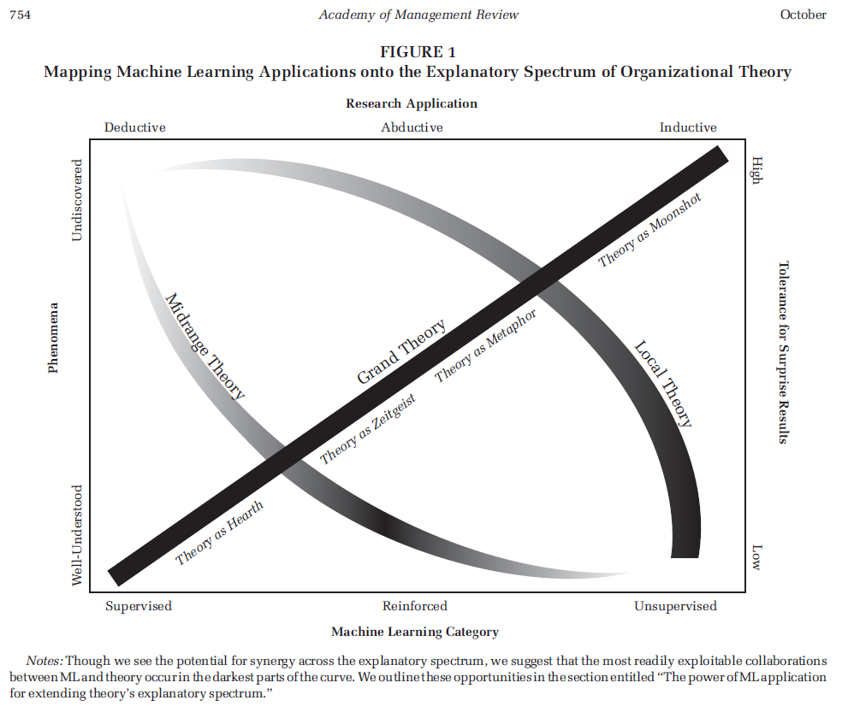
\includegraphics[width=0.75\linewidth]{figs/Leavitt_2021_Fig1.png}
		\caption{Source: \textcite[]{leavitt2021}}
		\label{fig:Leavitt_2021_Fig1}
	\end{figure}
\end{frame}


\begin{frame}
\frametitle{Data-driven Modeling in WOP}
\framesubtitle{Epistemological Considerations}
	{\footnotesize
	\begin{itemize}
		\item \textbf{Midrange Theory}: Explains specific phenomena with broader scope; detailed, applicable in various contexts. \textcolor{red}{Dominates organizational science; Further reinforcement of well-established	theories, instead of challenging already influential theories. Litany of constructs, models and theories that remain disconnected from one another.}
		\item \textbf{Local Theory}: Targeting urgent, pragmatic problems in the here and now.
		\item \textbf{Grand Theory}: Sufficiently expansive, bold, and generalizable across contexts and time to serve the discrete social-functional purposes of organizing and inspiring.
		\item \textbf{Theory as Hearth}: Central point of cohesion and stability; creates community, stable foundation.
		\item \textbf{Theory as Zeitgeist}: Reflects ideas of a specific period (``spirit of the time''); culturally influenced, can become obsolete.
		\item \textbf{Theory as Metaphor}: Uses metaphors to explain phenomena; facilitates understanding, inspires new thinking.
		\item \textbf{Theory as Moonshot}: Long-term, audacious goals that require new approaches to problem-solving.
    \end{itemize}
	}
\end{frame}


\begin{frame}
	\frametitle{From Theory Proliferation to Theory Integration}
	\framesubtitle{Inductive Approach for Integrating Performance Theories}
	\begin{itemize}
		\item<1-2> Do you know how many theories of Performance (Firm and Individual) we have?
		\item<2> According to Marshall, Aguinis, \& Beltran \parencite*{marshall2024theories_performance}, in organizational science there are \textbf{239 theories} about firm and individual performance (see also \cite{aguinis2024performance})
	\end{itemize}
	\only<3>{
	\vspace{-2.5cm} % Adjust this value to move the figure up, otherwise the "\only" forces the distance between title and figure accoring to the first slide (i.e., the slide defined by `<1>`)
	\begin{figure}
		\centering
		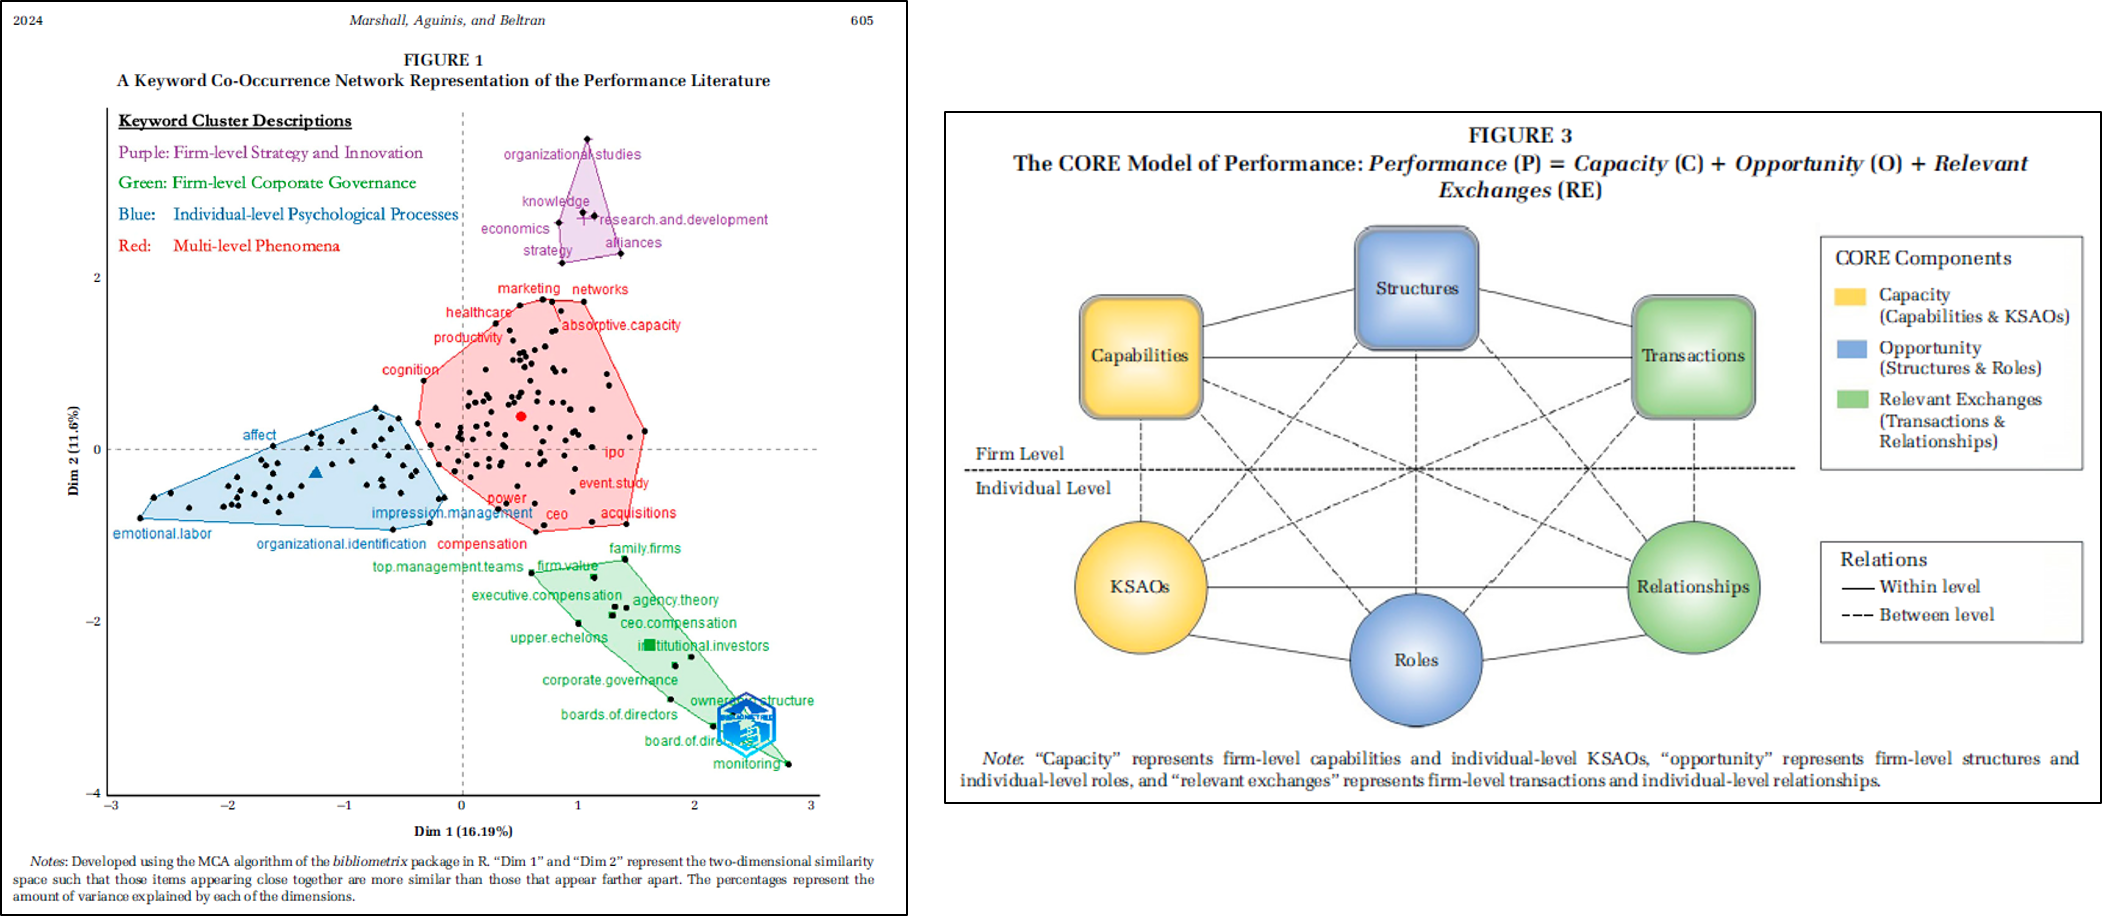
\includegraphics[width=1\linewidth]{figs/Marshall2024.png}
		\caption{{\scriptsize From \textbf{239 theories} to \textbf{4 keyword co-occurrence clusters} to \textbf{6 isomorphic meta-theoretical constructs}. \\
				Source: \textcite[p. 605 and p. 610]{marshall2024theories_performance}}}
		\label{fig:Marshall2024}
	\end{figure}
	}
\end{frame}



%%%%%%%%%%%%%%%%%%%%%%%%%% Integration

\section{Towards an integration}



\begin{frame}
	\frametitle{Do we need to integrate Theory-driven and Data-driven modeling in WOP Quantitative Research?}
	\framesubtitle{Some reasons}
	\only<1>{	
	\begin{itemize}
		\item It allows a better use of abductive reasoning, even in quantitative research methods: 
		\begin{itemize}
			\item Theories are reinforced, pruned, or merged; ``identifying conclusions that synthesize competing or previously disconnected theoretical findings or perspectives'' {\scriptsize \parencite[p. 19]{jacobucci2023machine}}.
			\item From data-driven to theory-driven models: Identifying robust empirical regularities and explaining them by abductively inferring underlying causal mechanisms {\scriptsize \parencite{haig2020bigData}}.
		\end{itemize}
	\end{itemize}
	}	
	\only<2>{
		\footnotesize
	\begin{itemize}
		\item Better integration between qual and quant research (e.g., in analyzing textual data; Banks et al., \cite*{banks2018_text}) and open the way to new assessment methods based on semantic/syntactic associations \parencite{stanghellini2024} \\
			\begin{figure}
				\centering
				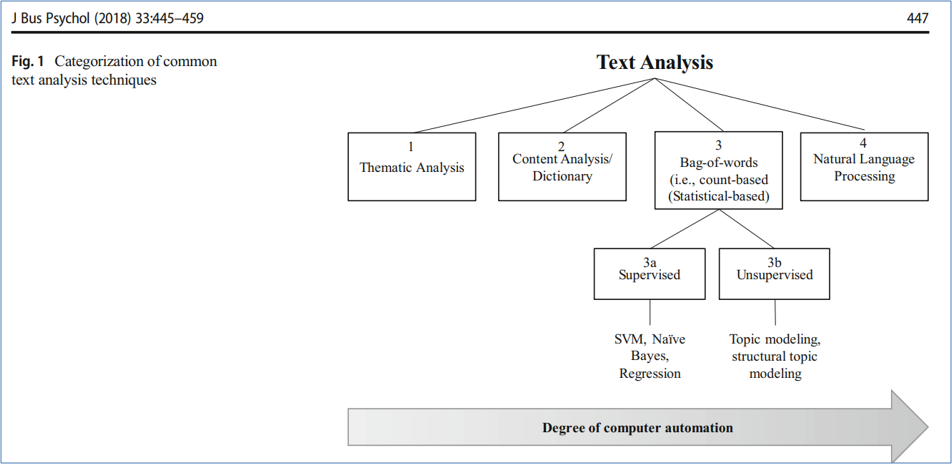
\includegraphics[width=0.9\linewidth]{figs/banks2018.png}
				\caption{{\tiny Source: \textcite[p. 447]{banks2018_text}}}
				\label{fig:banks2018}
			\end{figure}		
	\end{itemize}	
	}
\end{frame}


\begin{frame}
	\frametitle{The Rise of Hybrid Methodological Techniques}
	\framesubtitle{Some examples}
	\begin{itemize}
		\item Hybrid latent-variable machine-learning techniques, such as regularized SEM and SEM forests {\scriptsize \parencite{brandmaier2023machine, jacobucci2023machine}}
		\item Exploratory Mediation Analysis {\scriptsize \parencite{serang2017exploratoryMed}} 
		\item Deductive Data Mining {\scriptsize \parencite{hong2020deductive}} 
	\end{itemize}
\end{frame}


\begin{frame}
	\frametitle{A Note on Explainable Artificial Intelligence (XAI)}
	\framesubtitle{Beyond Black Boxes: Making Machine Learning Interpretable}
	\begin{columns}[c] 
		% Left column (1/2 of the width)
		\column{0.50\textwidth}
		{\small
		\begin{itemize}
			\item  Since 2017, the increasing development of techniques such as SHapley Additive exPlanations (\textbf{SHAP}) values, Partial Dependence Plots (\textbf{PDP}), and Accumulated Local Effects (\textbf{ALE}) Plots, has made the interpretation of ML results more interpretable {\scriptsize \parencite{molnar_XAI}}
			\item Application in WOP: Nonlinearity in personality–job performance relations {\scriptsize \parencite{song_XAI}}
		\end{itemize}
	}
	% Right column (2/2 of the width)
	\column{0.50\textwidth}
%	\vspace{-1cm} % Adjust this value as needed to move the figure up
	\begin{figure}
		\centering
		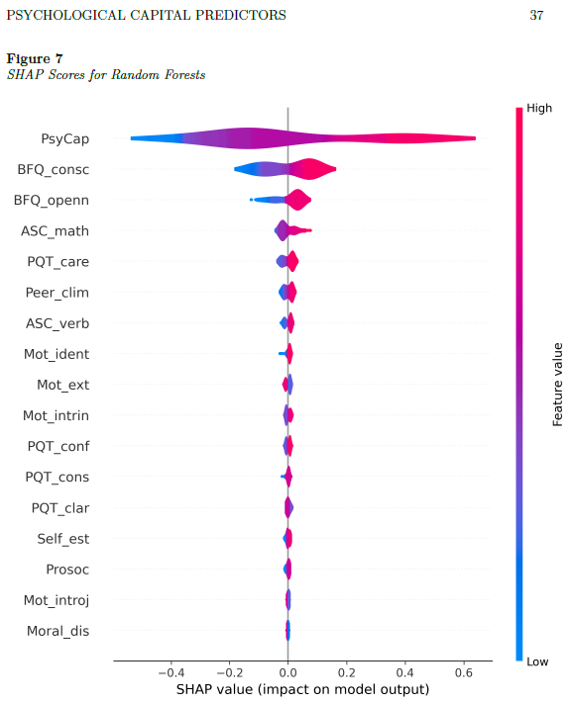
\includegraphics[width=0.8\linewidth]{figs/shap_PsyCap.png}
		\caption{{\scriptsize Lagged predictors of PsyCap levels at T2 (paper under review)}}
		\label{fig:shap_PsyCap}
	\end{figure}
	\end{columns}
\end{frame}


\begin{frame}
	\setbeamercovered{transparent}
	\frametitle{Conclusion}
	\framesubtitle{Removing Barriers}
	\begin{itemize}
		\item<1> Drawing from the work by \textcite{paxton2017}, we can outline \textbf{three gaps} that prevent the use and acceptance of these new sources of data and data-analyses:		
		\begin{itemize}
			\item<1> IMAGINATION GAP: the inability of researchers to see themselves, their research area, and their specific research question under (quantitative) inductive methods
			\item<1> CULTURE GAP: lack of acceptance of these approaches
			\item<1> SKILLS GAP: new tools, methods, and analyses to learn {\scriptsize \parencite{konig2020advice, landers2019data}}			
		\end{itemize}		
	\item<2> In sum, many of the concerns can be overcome by recognizing two types of problems:
		\begin{itemize}
			\item<2> EPISTEMOLOGICAL: Clearly specify the epistemological position of both the research question and the data to be analyzed.
			\item<2> TECHNICAL: Enhance technical skills in programming languages (e.g., R and Python) and develop proficiency in novel data analytic strategies (e.g., XAI, NLP, etc.).
		\end{itemize}
	\end{itemize}
\end{frame}


\begin{frame}
	\setbeamercovered{transparent}
	\frametitle{Conclusion}
	\framesubtitle{The Future I See}
	{\small
		\begin{itemize}
			\item<1> The role of Subject Matter Experts (SMEs) remains pivotal, as the validation of these approaches is and will continue to be essential {\scriptsize \parencite{woo2024}}.
			\item<2> Increased convergence and exchange between Quant and Qual methods {\scriptsize \parencite[see][]{bliese2024_AOM}}.
			\item<3> Greater emphasis on formalizing (quantitative) theories from computational and mathematical perspectives {\scriptsize \parencite{bliese2024_AOM, grand_inPressORM, vanDongen_inPress_PsychReview}}. E.g., is the JD-R theory robust enough for predictive approaches?
			\item<4> Job Analysis: A cornerstone of WOP with a long history {\scriptsize \parencite{viteles1922}}, but it has received limited attention in recent research {\scriptsize \parencite{li2024jobAnalysis, putka2023evaluating}}. Could LLMs and predictive models help bridge the scientist-practitioner gap?
			\item<5> Advancing studies on Performance Management Systems and related theories (e.g., predictions/outcomes of performance instability).
		\end{itemize}
	}
\end{frame}


%%%%%%%%%%%%%%%%%%%%%%%%%% References

\begin{frame}[allowframebreaks]{References}
    \printbibliography
\end{frame}


%%%%%%%%%%%%%%%%%%%%%%%%%% Final slide

\begin{frame}
	\huge	
	\begin{center}
		Thanks for your attention	     
	\end{center}
	\normalsize
	\begin{center}
		\href{mailto:enrico.perinelli@unitn.it}{\nolinkurl{enrico.perinelli@unitn.it}} \\
		\vspace{20pt}
		{\tiny Presentation available at \\
			 \texttt{\url{https://github.com/EnricoPerinelli/AIP-2024_YoungKeynote/blob/master/AIP_2024_YoungKeynote.pdf}}
			 }
		\begin{figure}
			\centering
			
\includegraphics[width=0.25\linewidth]{figs/qr-code_github.png}
%			\caption{}
			\label{fig:qr_code}
		\end{figure}
		\begin{tikzpicture}[remember picture, overlay]
			% Left image
			\node[opacity=1, inner sep=1pt] at ([xshift=2.2cm,yshift=1.5cm]current page.south west) {
				
\includegraphics[height=0.1\paperheight]{figs/logoDIPSCO.png}
			};
			% Right image
			\node[opacity=1, inner sep=1pt] at ([xshift=-2.2cm,yshift=1.5cm]current page.south east) {
				
\includegraphics[height=0.1\paperheight]{figs/logoAIP.png}
			};
		\end{tikzpicture}
	\end{center}
\end{frame}


%%%%%%%%%%%%%%%%%%%%%%%%%% End document

\end{document}
